% !TEX TS-program = pdflatex
% !TEX root = RicOp2.tex

\documentclass[a4paper,twoside,openright,titlepage,
               headinclude,,footinclude,BCOR5mm,
               numbers=noenddot,cleardoublepage=empty,
               tablecaptionabove]{scrreprt}
               
\usepackage[T1]{fontenc}
\usepackage[utf8]{inputenc}
\usepackage[english]{babel}
\usepackage{amsmath,amssymb}
\usepackage{indentfirst}
\usepackage[style=philosophy-modern,hyperref]{biblatex}
%\usepackage{biblatex}
\addbibresource{Bibliography.bib}
\usepackage{chngpage}
\usepackage{multirow}
\usepackage{calc}
\usepackage{listings}
\usepackage{graphicx}
\usepackage{subfig}
\usepackage{lipsum}
\usepackage{shapepar}
\usepackage{pifont}
\usepackage[eulerchapternumbers,subfig,beramono,eulermath,pdfspacing,listings]{classicthesis}
\usepackage{arsclassica}
\usepackage{tabto}
%\usepackage{minitoc}

% ********************************************************************
% Personal commands
% ******************************************************************** 
\newcommand{\myName}{Lorenzo Pantieri}
\newcommand{\myTitle}{The ArsClassica package}
\newcommand{\mySubTitle}{Ah homage to the Elements of Typographic Style}

\DeclareRobustCommand*{\clsname}[1]{{\normalfont\sffamily#1}}
\DeclareRobustCommand*{\pkgname}[1]{{\normalfont\sffamily#1}}
\DeclareRobustCommand*{\optname}[1]{{\normalfont\ttfamily#1}}
\DeclareRobustCommand*{\cmdname}[1]{\mbox{\lstinline[basicstyle=\normalsize\ttfamily]!\\#1!}}

\DeclareRobustCommand*{\classicthesis}{Classic\-Thesis}
\DeclareRobustCommand*{\arsclassica}{{\normalfont\sffamily ArsClassica}}


% ********************************************************************
% Hyper-references
% ******************************************************************** 
\newcommand{\mail}[1]{\href{mailto:#1}{\texttt{#1}}}


% ********************************************************************
% Graphics
% ********************************************************************
\graphicspath{{Graphics/}}


% ********************************************************************
% Code
% ********************************************************************
\definecolor{lightergray}{gray}{0.99}

\lstset{language=[LaTeX]Tex,
     keywordstyle=\color{RoyalBlue},
     basicstyle=\small\ttfamily,
     commentstyle=\color{Emerald}\ttfamily,
     stringstyle=\rmfamily,
     numberstyle=\scriptsize,
     showstringspaces=false,
     breaklines=true,
     frame=lines,
     backgroundcolor=\color{lightergray},
     flexiblecolumns=true,
     escapeinside={�*}{*�},
     firstnumber=last,
} 

\newcommand{\meta}[1]{$\langle${\normalfont\itshape#1}$\rangle$}

\lstset{	morekeywords=%
    {ProvidesPackage,RequirePackage,areaset,ifthenelse,%
     chapterNumber,undefined,boolean,DeclareRobustCommand,%
     spacedallcaps,textssc,MakeTextUppercase,lehead,%
     microtypesetup,textls,spacedlowsmallcaps,MakeTextLowercase,%
     sodef,allcapsspacing,lowsmallcapsspacing,thesection,%
     color,headmark,rohead,headfont,pnumfont,titleformat,%
     part,partname,thepart,chapter,thechapter,titlerule,%
     subsection,thesubsection,subsubsection,thesubsubsection,%
     paragraph,theparagraph,descriptionlabel,titlespacing,%
     formatchapter,textcolor,clearscrplain,rofoot,labelitemi,
     captionsetup,hypersetup}}

\lstnewenvironment{code}% 
   {\setkeys{lst}{columns=fullflexible,keepspaces=true}%
   \lstset{basicstyle=\small\ttfamily}}{}


% ********************************************************************
% Bibliography
% ******************************************************************** 
\bibliography{Bibliography}

\defbibheading{bibliography}{%
\cleardoublepage
\manualmark
\phantomsection
\addcontentsline{toc}{chapter}{\tocEntry{\bibname}}
\chapter*{\bibname\markboth{\spacedlowsmallcaps{\bibname}}
{\spacedlowsmallcaps{\bibname}}}}

\renewcommand*{\nameyeardelim}{\addcomma\space}

\begin{document}
%\dominitoc
%\dominilof
%\dominilot
%\faketableofcontents
%\fakelistoffigures
%\fakelistoftables
\pagenumbering{roman}
\pagestyle{plain}
% !TEX TS-program = pdflatex
% !TEX root = ../ArsClassica.tex
%*******************************************************
% Titlepage
%*******************************************************
\begin{titlepage}
\pdfbookmark{Titlepage}{Titlepage}
\changetext{}{}{}{((\paperwidth  - \textwidth) / 2) - \oddsidemargin - \hoffset - 1in}{}
    \begin{center}

	\begin{center}
	
\includegraphics[scale=0.08]{Graphics/unipd.png}
	\end{center}
	
	\vspace{0.2in}	
	\textsc{\LARGE Università degli Studi di Padova}\\[1.5cm]
    \vspace{1.3in}
    \Huge \textmd{\textbf{Wind Farm Cable Problem}}\\
	\vspace{0.1in}   
    \Large Advanced combinatorial optimization algorithms \\
    \Large Ricerca Operativa 2\\
    \vspace{1in}
	\NumTabs{6}
	\begin{minipage}{5cm} 
	\centering
	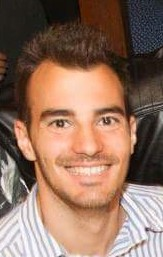
\includegraphics[scale=0.5]{Graphics/Foto.jpg} \\
	\textbf{Piona Davide} \\	
	\textbf{1149616}
	\end{minipage}
	\begin{minipage}{5cm} 
	\centering
	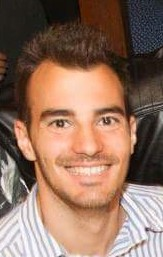
\includegraphics[scale=0.5]{Graphics/Foto.jpg} \\
	\textbf{Benini Michele} \\	
	\textbf{1139089}
	\end{minipage}
 	\vspace{1in}
 	\\	
	\Large Academic Year 2017-2018\\
	
  	                    

    \end{center}        
\end{titlepage} 
%% !TEX TS-program = pdflatex
% !TEX root = ../ArsClassica.tex

%*******************************************************
% Titleback
%*******************************************************
\thispagestyle{empty}
\pdfbookmark{Titleback}{Titleback}

\hfill

\vspace{\stretch{2}}

\begin{center}
Lorenzo Pantieri \\
\smallskip
\textit{The \arsclassica{} package}\\
\smallskip
Copyright\,\textcopyright\ 2008-2017
\end{center}
\vspace{\stretch{1}}

\medskip

\noindent\textsf{\spacedlowsmallcaps{Titleback}} \\
\noindent
This document was written with \LaTeX{} on Mac using \arsclassica, a reworking of the \classicthesis{} style designed by Andr\'e Miede, inspired to the masterpiece \emph{The Elements of Typographic Style} by Robert Bringhurst. 

\bigskip

\noindent
\textsf{\spacedlowsmallcaps{Contacts}}

\noindent
{\raisebox{-0.33ex}{\ding{43}}}\,\mail{lorenzo.pantieri@gmail.com}
\cleardoublepage
\pagestyle{scrheadings} 
% !TEX TS-program = pdflatex
% !TEX root = ../ArsClassica.tex

%*******************************************************
% Contents
%*******************************************************
\phantomsection
\pdfbookmark{\contentsname}{tableofcontents}
\setcounter{tocdepth}{2}
\tableofcontents
\markboth{\spacedlowsmallcaps{\contentsname}}{\spacedlowsmallcaps{\contentsname}} 
\cleardoublepage
\pagenumbering{arabic}
%% !TEX TS-program = pdflatex
% !TEX root = ../ArsClassica.tex

%************************************************
\chapter{Fundamentals}
\label{chp:fundamentals}
%************************************************

This chapter introduces the (truly simple) basic notions of \arsclassica{} and presents its fundamental ideas and distinctive features.



\section{Introduction}

The \arsclassica{} package changes some features of the \classicthesis{} style, designed by Andr\'e Miede. It allows to reproduce the layout of the \LaTeX{} guide \emph{The Art of Writing with \LaTeX}~\parencite{pantieri:arte} and of this document.

\section{Use}

This package is shaped to be executed on a \emph{complete} installation of \TeX{}~Live or MiK\TeX, and uses freely available fonts.
It works with the \clsname{KOMA-Script} classes (\clsname{scrreprt}, \clsname{scrbook} and \clsname{scrartcl}) and requires the \pkgname{classicthesis} package. \arsclassica{} must be loaded \emph{after} \pkgname{classicthesis}:
\begin{code}
\documentclass[�*\meta{\dots\unkern}*�]{scrreprt} % or scrbook or scrartcl

\usepackage[�*\meta{\dots\unkern}*�]{classicthesis}
\usepackage{arsclassica}

\begin{document}
�*\dots*�
\end{document}
\end{code}

For example, this document has been produced with the following code:
\begin{code}
\documentclass[a4paper,twoside,openright,titlepage,
               headinclude,footinclude,BCOR5mm,
               numbers=noenddot,cleardoublepage=empty,
               tablecaptionabove]{scrreprt}

\usepackage{�*\meta{\dots\unkern}*�}
\usepackage{subfig}
\usepackage[eulerchapternumbers,subfig,beramono,eulermath,pdfspacing]%
           {classicthesis}
\usepackage{arsclassica}

\begin{document}
�*\dots*�
\end{document}
\end{code}

It is recommended to use the \optname{beramono} and \optname{eulerchapternumbers} options together with \arsclassica.



\section{Style}

The typographical style achieved with \arsclassica{} differs from \classicthesis{} in the following points:
\begin{itemize}
\item use of Iwona font, by Janusz Nowacki, for the sectioning unit titles (chapters, sections, subsections, sub-subsections, paragraphs and subparagraphs), for the description list labels, the headlines and the caption labels (\classicthesis{} doesn't use any sans serif font);
\item customized chapter numbers;
\item semi-transparent headlines; the headlines are separated from the page number by a small rule;
\item caption labels in boldface (\classicthesis{} doesn't use any boldface font);
\item itemize lists with semi-transparent bullets.
\end{itemize}

\arsclassica{} is designed  to provide a ready-to-use typographical style: for this reason it has no loading options and it is \emph{not} configurable or customizable in any way. If you change the previous settings, you'll risk to destroy the balance of the style, so it is \emph{highly recommended} to keep them unchanged.

One of the principles of \LaTeX{} is that it allows the author to take no interest in the typographical questions, permitting him to focus only on the structure and the contents of his document. This fact should always be kept in mind: using a style written by others, the user accepts all the typographical settings chosen for him by the author of the style, and he isn't forced to study typography to fine-tune the layout of his publications. This is the case of \arsclassica{} too: if you change its settings, you'll deny this philosophy and, consequently, you'll have to study (a lot of) typography to achieve acceptable results. 

The style achieved with \arsclassica{} is \emph{not} therefore configurable or customizable. The typographical style is very personal: if you like this package and find attractive the idea to take no interest in the problem of the style definition, then you'll use \arsclassica{} with satisfaction; otherwise, if you have different needs or you aren't satisfied with the layout of the package, then you should try other classes or packages, even building your own style.



\section{Important}

To write a document according to the \arsclassica{} style, you have to follow some very simple rules.
\begin{itemize}
\item Don't change \emph{for any reason} the \arsclassica{} settings (fonts, text body size, colors, \dots).
\item The sectioning unit titles (chapters, section, subsections, \dots) have to be \emph{one line long}, possibly in \emph{plain text} (no symbols, formulas or code fragments). If you have titles longer than one line, try and rephrase them: you can almost always do it.
\item In the table of contents and in the list of tables and figures, captions have to be \emph{one line long}, possibly in \emph{plain text}. Use the optional argument of sectioning commands and of \cmdname{caption}, if necessary.
\item Don't use \optname{tocaligned} and \optname{dottedtoc} options of \classicthesis: the default table of contents does the job very well (see the documentation of \classicthesis{} for a nice discussion of this point).
\item Don't use vertical or double rules in your tables (see the documentation of \pkgname{booktabs}).
\item Use footnotes and margin notes very sparingly.
\item If your document includes graphs and plots, draw them using \LaTeX{} (by \pkgname{Ti\emph{k}Z} and \pkgname{pgfplots}, for example) and not an external software. This is the only way to get the best typographical outcome. 
\end{itemize}


 
\section{Examples}

\begin{figure}
\centering
\subfloat[Asia personas duo]
{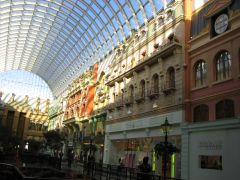
\includegraphics[width=.45\columnwidth]{Lorem}} \quad
\subfloat[Pan ma signo]
{\label{fig:example-b}%
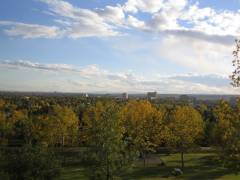
\includegraphics[width=.45\columnwidth]{Ipsum}} \\
\subfloat[Methodicamente o uno]
{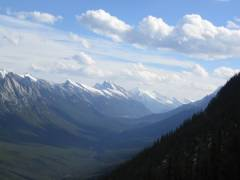
\includegraphics[width=.45\columnwidth]{Dolor}} \quad
\subfloat[Titulo debitas]
{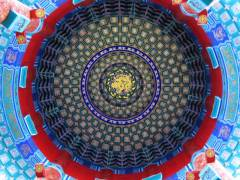
\includegraphics[width=.45\columnwidth]{Sit}}
\caption[Tu duo titulo debitas latente]{Tu duo titulo debitas latente}
\label{fig:example}
\end{figure}

Please note that the content of this section is just some dummy text. It isn't a real language.

Lorem ipsum dolor sit amet, consectetuer adipiscing elit. Ut purus elit, vestibulum ut, placerat ac, adipiscing vitae, felis. Curabitur dictum gravida mauris.

\subsection*{A subsection}

\lipsum[2]

\subsubsection*{A sub-subsection}

\lipsum[7]

\paragraph{A paragraph}
Lorem ipsum dolor sit amet, consectetuer adipiscing elit. Ut purus elit, vestibulum ut, placerat ac, adipiscing vitae, felis. Curabitur dictum gravida mauris. Nam arcu libero, nonummy eget, consectetuer id, vulputate a, magna.

\paragraph{Another paragraph}
Cras nec ante, pellentesque a nulla, cum sociis natoque penatibus et magnis dis parturient montes, nascetur ridiculus mus. Aliquam tincidunt urna

\bigskip

Donec aliquet, tortor sed accumsan bibendum, erat ligula aliquet magna, vitae ornare odio metus a mi. Morbi ac orci et nisl hendrerit mollis. Suspendisse ut massa. Cras nec ante. Pellentesque a nulla. Cum sociis natoque penatibus et magnis dis parturient montes, nascetur ridiculus mus. Aliquam tincidunt urna.

\begin{description}
\item[Mane] Lorem ipsum dolor sit amet, consectetuer adipiscing elit. 
\item[Tekel] Ut purus elit, vestibulum ut, placerat ac, adipiscing vitae, felis. Curabitur dictum gravida mauris.
\item[Fares] Nam arcu libero, nonummy eget, consectetuer 
id, vulputate a, magna.
\end{description}

\begin{table}
\caption{Lorem ipsum dolor sit amet}
\centering
\begin{tabular}{ll}
\toprule
\textbf{Alkaloid} & \textbf{Origin} \\
\midrule
atropine & belladonna \\
morphine & poppy \\
nicotine & tobacco \\
\bottomrule
\end{tabular}
\end{table}

Suspendisse vel felis. Ut lorem lorem, interdum eu, tincidunt sit amet, laoreet vitae, arcu. Aenean faucibus pede eu ante. Praesent enim elit, rutrum at, molestie non, nonummy vel, nisl. Ut lectus eros, malesuada sit amet, fermentum eu, sodales cursus, magna. Donec eu purus. Quisque vehicula, urna sed ultricies auctor, pede lorem egestas dui, et convallis elit erat sed nulla.

\subsection*{Some formulas}

Una formula in linea viene incorporata nel testo: $\lim_{n \to \infty}\sum_{k=1}^n \frac{1}{k^2} = \frac{\pi^2}{6}$, per esempio. Come si osserva, \LaTeX{} fa \emph{il possibile} per comprimerla e modificare il meno possibile l'interlinea nel capoverso che la contiene.
Una formula in display viene invece composta da \LaTeX{} su linee a parte, separate dal contesto con adeguati spazi bianchi per metterla in mostra e farla risaltare sulla pagina.
\begin{equation}
\lim_{n \to \infty}\sum_{k=1}^n \frac{1}{k^2}= \frac{\pi^2}{6}
\end{equation}
Come si osserva, ora la formula risulta centrata, non compressa, e tutti i suoi elementi occupano il giusto spazio con un risultato finale di grande respiro.

Integer tempus convallis augue. Etiam facilisis. Nunc elementum fermentum wisi. Aenean placerat. Ut imperdiet, enim sed gravida sollicitudin, felis odio placerat quam, ac pulvinar elit purus eget enim. 

\begin{equation}
\int_a^{a+T}f(x)\,dx= \int_0^T f(x)\,dx 
\qquad
\oint f(z)\,dz=2\pi i
\end{equation}

Nulla malesuada porttitor diam. Donec felis erat, congue non, volutpat at, tincidunt tristique, libero. Vivamus viverra fermentum felis. Donec non- ummy pellentesque ante.

\begin{equation}
f(x_1,\dots,x_n)=  \prod_{k=1}^n x_k 
\qquad
\sum_{k=1}^n x_k^2=1
\qquad
\biggl(\sum_n x_n^2\biggr)^{1/2} 
\end{equation}

\lipsum[2]

\begin{equation}
\begin{bmatrix} 
a_{11} & \dots & a_{1n} \\ 
a_{21} & \dots & a_{2n} \\ 
\hdotsfor{3} \\ 
a_{n1} & \dots & a_{nn} 
\end{bmatrix}
\end{equation}

\lipsum[4]

\begin{equation}
\lim_{x\to 0}
\frac{\sin x}{x}=1 \qquad
\lim_{n\to +\infty}f_n=\delta
\end{equation}

Fusce mauris. Vestibulum luctus nibh at lectus. Sed bibendum, nulla a faucibus semper, leo velit ultricies tellus, ac venenatis arcu wisi vel nisl. Vestibulum diam.

\begin{equation}
n!=
\begin{cases} 
1       & \text{if $n=0$} \\ 
n(n-1)! & \text{if $n\ge 1$} 
\end{cases} 
\end{equation}

Ut lectus eros, malesuada sit amet, fermentum eu, sodales cursus, magna. Donec eu purus. Quisque vehicula, urna sed ultricies auctor, pede lorem egestas dui, et convallis elit erat sed nulla. Donec luctus. Curabitur et nunc. Aliquam dolor odio, commodo pretium, ultricies non, pharetra in, velit.

\begin{equation} 
x_G=
\frac{\displaystyle
      \sum_{i=1}^n m_ix_i}
{\displaystyle\sum_{i=1}^n m_i}
\end{equation}

\lipsum[6]

\begin{equation}
\kappa =\frac{\xi}{E_{\textrm{max}}}
\qquad
E_{\textup{max}} =\frac{2 m_{\textup{e}} \beta^2\gamma^2 }{1 +2\gamma m_{\textup{e}}/m_{\textrm{x}} + ( m_{\textup{e}}/m_{\textup{x}})^2}
\end{equation}

\lipsum[8]
% !TEX TS-program = pdflatex
% !TEX root = ../ArsClassica.tex

%************************************************
\chapter{Development Environment}
\label{chp:1-Environment}
%************************************************
To allow replicability of our experiments, we have added some information about the system and the environment that we used for our research. 
We used the following development environment:
\begin{itemize}
\item \textsc{CPLEX} :  version 0.1-2018
\item \textsc{Linux Ubuntu} : version 18.04 LTS (Operative System)
\item \textsc{C}  	(language)
\item \textsc{Sublime text} (IDE / text editor)
\item \textsc{Github} (web-based version control using Git)
\item \textsc{Gnuplot} (library plot)
\end{itemize}

\section{Real World Info}
As in [\cite{wfcp}] research, we used a library of real-life instances that are publicly available for benchmarking.
For benchmark purposes, we collected the data of five real wind farms in operation in United Kingdom (wf02, wf03, wf05) and Denmark (wf01, wf04). Different types of cable with different costs, capacities and electrical resistances are available on the market; we considered 5 sets of real cables, named cb01, cb02, cb03, cb04, and cb05. The turbines in each wind park are of the same type, so we can express the cable capacities as the maximum number of turbines that it can support. Finally, we list the maximum number of connections to the substation, or to be specific, the input parameter C. The table 1 contains all the information.
\begin{table}[!htbp]\label{tab:realWorld}
\center
\begin{tabular}{llllll}
\hline
name & site         & turbine type  & no. of turbines & C  & allowed cables      \\ \hline
wf01 & Horn Rev 1   & Vestas 80-2MW & 80              & 10 & cb01-cb02-cb05      \\
wf02 & Kentis Flats & Vestas 90-3MW & 30              & $\infty$   & cb01-cb02-cb04-cb05 \\
wf03 & Ormonde      & Senvion 5MW   & 30              & 4  & cb03-cb04           \\
wf04 & DanTysk      & Simens 3.6MV  & 80              & 10 & cb01                \\
wf05 & Thanet       & Vestas 90-3MW & 100             & 10 & cb04-cb05           \\ \hline
\end{tabular}
\caption{Basic information on the real-world wind farms that were used for testing.}
\end{table}

\section{Instance TEST BED}
The test that we were able to use are the combinations between the 5 instances of wind farms and the 5 sets of real cables. For simplicity reasons and in order to eliminate mistakes, we adopted the same a numeration as the [\cite{wfcp}] article. This solution allows us to easily compare our results with the results in that research. 
Table 2 reports the resulting numbers of the different instances. For example we renamed the 01 wind farm as \textit{data\_01.turb} and the corresponding cables as \textit{data\_01.cbl}. Figures \ref{img:ex1} and \ref{img:ex2} shows two instances from TEST BED.

\begin{table}[!htbp]\label{tab:testBed}
\center
\begin{tabular}{lcl}
\hline
number & \multicolumn{1}{l}{wind farm} & cable set         \\ \hline
01     & \multirow{6}{*}{wf01}         & wf01\_cb01\_capex \\
02     &                               & wf01\_cb01        \\
03     &                               & wf01\_cb02\_capex \\
04     &                               & wf01\_cb02        \\
05     &                               & wf01\_cb05\_capex \\
06     &                               & wf01\_cb05        \\ \hline
07     & \multirow{8}{*}{wf02}         & wf02\_cb01\_capex \\
08     &                               & wf02\_cb01        \\
09     &                               & wf02\_cb02\_capex \\
10     &                               & wf02\_cb02        \\
12     &                               & wf02\_cb04\_capex \\
13     &                               & wf02\_cb04        \\
14     &                               & wf02\_cb05\_capex \\
15     &                               & wf02\_cb05        \\ \hline
16     & \multirow{4}{*}{wf03}         & wf03\_cb03\_capex \\
17     &                               & wf03\_cb03        \\
18     &                               & wf03\_cb04\_capex \\
19     &                               & wf03\_cb04        \\ \hline
20     & \multirow{2}{*}{wf04}         & wf04\_cb01\_capex \\
21     &                               & wf04\_cb01        \\ \hline
26     & \multirow{4}{*}{wf05}         & wf05\_cb04\_capex \\
27     &                               & wf05\_cb04        \\
28     &                               & wf05\_cb05\_capex \\
29     &                               & wf05\_cb05        \\ \hline
\end{tabular}
\caption {Test Bed instance numbers.}
\end{table}

\begin{minipage}{7cm} 
	\centering
	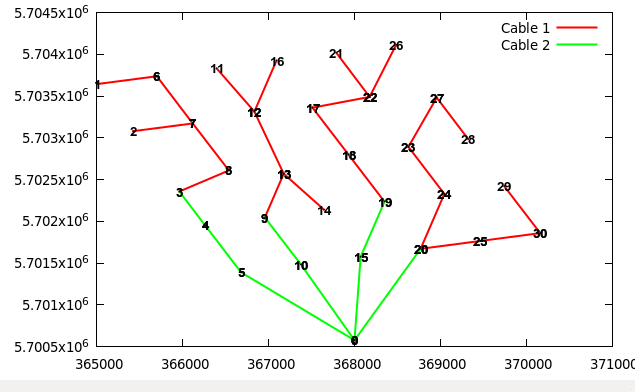
\includegraphics[scale=0.3]{Graphics/data07.png} \\
	\captionof{figure}{Example of problem: data07}
	\label{img:ex1}
	\end{minipage}
	\begin{minipage}{7cm} 
	\centering
	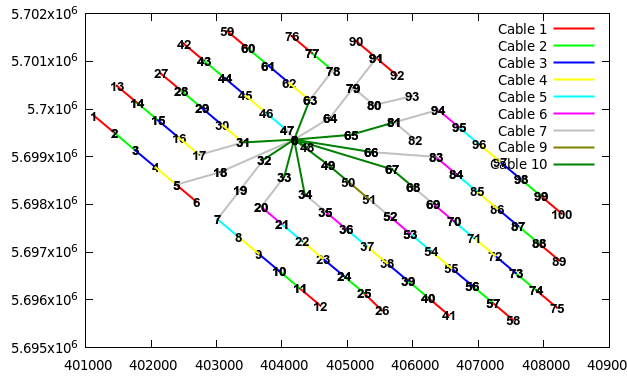
\includegraphics[scale=0.3]{Graphics/data29.png} \\
	\captionof{figure}{Example of problem: data29}
	\label{img:ex2}
	\end{minipage}

\newpage
% !TEX TS-program = pdflatex
% !TEX root = ../ArsClassica.tex

%************************************************
\chapter{Mathematical Model}
\label{chp:2-Model}
%************************************************

\section{Wind Farm Cable Problem Introduction}
We have studied the Wind Farms Cable Problem, which is represented by a number of wind farms in the sea that produces energy; the power production needs to be routed by some cables to the substation and then directed to the coast.
To do that, each turbine must be connected through a cable to another turbine, and eventually to a substation.\\

The problem complexity of the cable routing problem is strongly NP-hard according to \cite{wfcp}. They have proved that the problem is NP-hard in two formulations. First, in the case where all turbines have the same power production and the nodes are not associated with points in the plane. Second, in the case where the turbines can have different power production and are associated with point in the plane. 

When designing a feasible cable routing, it's necessary to take in account a number of constraints. Here we list some of them and then we'll describe the mathematical model that realizes those constraints. Our model is based on the following requirements:

\begin{itemize}
\item since the energy flow is unsplittable, the energy flow leaving a turbine must be supported by a single cable.
\item power losses should be avoided because it will cause revenue losses in the future.
\item different cables, with different capacities and costs are available. This means that it is important to choose the right cable to minimize the costs without affecting the revenues. 
\item the energy flow on each connection cannot exceed the capacity of the installed cable.
\item due to the substation physical layout, a given maximum number of cables, say $C$, can be connected to each substation.
\item cable crossing should be avoided. (we will discuss this problem in the next subsection)
\end{itemize}
Let $K$ denote the number of different types of cables that can be used and let $n$ be the number turbines. 

Definition of $y_{ij}$ :
\[
	y_{ij} =
   \begin{cases}
   1 \quad \mbox{if arc } (i,j) \mbox{ is constructed} \\
   0 \quad \mbox{otherwise.} 
   \end{cases}
   \forall \,i,j = 1, ..., n 
\]
\[
	y_{ii} = 0, \quad \forall i= 1, ... n 
\]
Definition of $x^k_{ij}$ :
\[
	x^k_{ij} =
   \begin{cases}
   1 \quad \mbox{if arc } (i,j) \mbox{ is constructed with cable type k} \\
   0 \quad \mbox{otherwise.} 
   \end{cases}
   \forall \,i,j = 1, ..., n \ \forall \ k = 1,... K
\]
Definition of $f_{ij}$ :
\[
	f_{ij} \geq 0, \quad \forall i,j= 1, ... n
\]

%\[
%y_{i,j} = \sum_{t \in T} x^t_{ij}, \quad (i,j) \in A
%\]
Objective function: 
\begin{equation}\label{eq:obj}
	\min{\sum^n_{i=1} \sum^n_{j=1} \sum^K_{k} cost(k) \cdot dist(i,j) \cdot x^k_{ij}}
\end{equation}

Constraints: 
\begin{equation}\label{eq:numberCable}
	\sum^n_{j = 1} y_{hj} = 
	\begin{cases}
   1 \quad \mbox{if } P_h \geq 0, \quad \forall h=1,...,n \\
   0 \quad \mbox{if } P_h = -1
   \end{cases}
\end{equation}

\begin{equation}\label{eq:basestation}
	\sum^n_{i =1} y_{ih} \leq C, \quad \forall h \ | \ P_h = -1
\end{equation}

\begin{equation}\label{eq:flux}
	\sum^n_{j=1} f_{hj} = \sum^n_{i=1} f_{ih}+ P_h, \quad \forall h \ | \ P_h \geq 0
\end{equation}

\begin{equation}\label{eq:oneCable}
	y_{ij} = \sum^K_{k=1} x^k_{ij}, \quad i,j = 1,...,n
\end{equation}

\begin{equation}\label{eq:capacity}
	\sum^K_{k=1} cap(k)x^k_{ij} \geq f_{ij}, \quad \forall i,j = 1,...,n
\end{equation}

The objective function \ref{eq:obj} minimizes the total cable layout cost, where $dist(i, j)$ is the Euclidean distance between nodes $i$ and $j$ and $cost(k)$ is the unit cost for the cable $k$. 
Constraints \ref{eq:oneCable} impose that only one type of cable can be selected for each build arc.
Constraints \ref{eq:flux} are flow conservation constraints: the energy exiting each node $h$ is equal to the energy entering $h$ plus the power production of the node. 
Constraints \ref{eq:capacity} ensure that the flow does not exceed the capacity of the installed cable.
Constraints \ref{eq:numberCable} impose that only one cable can exit a turbine and that no one cable can exit from the substation. 
Constraint \ref{eq:basestation} imposes the maximum number of cables ($C$) that can enter in a substation, depending on the data of the instance. The image \ref{img:wfcp} shows an example of a graphical solution to the cable routing problem.

\begin{center}
	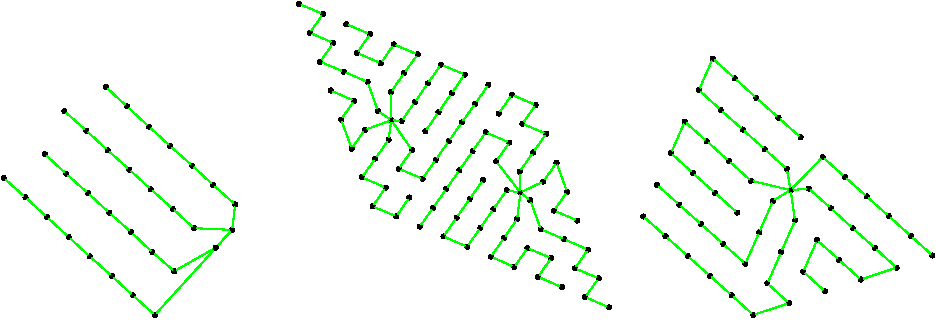
\includegraphics[scale=0.4]{Graphics/wfcp.png}
	\captionof{figure}{Example solutions to a cable routing problem}
	\label{img:wfcp}
\end{center}
	
\section{Crossing Cables}
According to \cite{wfcp}, an important constraint is that cable crossings should be avoided. In principle, cable crossing is not impossible, but is strongly discouraged, in practice as building one cable on top of another is more expensive and increases the risks of cable damages.\\

In order to evaluate if two arches cross, we used the Cramer Method: given the arc $a$ between $P_1$ and $P_2$ and the arc $b$ between $P_3$ and $P_4$. We define the coordinates of a general point as: $P_j = (X_i, y_i)$. \\
Using the Cramer method we have:
\[
{x \choose y} = {x_1 \choose y_1}+ \lambda {x_2 - x_1 \choose y_2 - y_1} \quad \lambda \in \ ]0, 1[
\]   
\[
{x \choose y} = {x_3 \choose y_3}+ \mu {x_4 - x_3 \choose y_4 - y_3} \quad \mu \in \ ]0, 1[
\]    
Then we evaluate if the determinant is equal to zero value. By using a calculator we will check if the determinant is smaller than a constant epsilon with value $\simeq 10^{-9}$. We can have two situations:
\begin{enumerate}
\item if $det=0 \quad \Rightarrow$ no crossing 
\item if $det \neq 0 \quad \Rightarrow (\lambda, \mu) \ if \ (\lambda \in \ ]0, 1[) \ \&\& \ (\mu \in \ ]0, 1[) \Rightarrow $ crossing
\end{enumerate}                                                   

\[
y(a,b)+ y(c,d) \leq 1, \quad \forall (a,b,c,d): [P_a, P_b] \ cross \ [P_c, P_d]
\]


% !TEX TS-program = pdflatex
% !TEX root = ../ArsClassica.tex

%************************************************
\chapter{Methods}

\label{chp:3-Methods}

%************************************************
\section{Plain Execution}
We simply create the linear programming model and then we pass it to CPLEX for the optimization. The performances, as we will notice for all the methods, depends on the instance: we noticed the power of CPLEX that find the optimal solution in few seconds, and in the meantime we discovered that some instances takes many hours to be solved by our machines. 
The main steps of our code in this phase are: 
to read the input files and parse it
...

\section{Relaxed Mode}
RELAX: this method tries to ‘relax’ some constraints in order to make faster the process of searching the first solution (so that RINS can start working). We add a slack variable >=0 in the model. Then we add this variable also in the objective function multiplied for a constant reasonably large. In this way, even if CPLEX could find a wrong initial solution, it’s probable that this solution will rapidly get better and became correct. 
\section{CPLEX Heuristics-Params}
We enable some CPLEX heuristic methods adapting them to our specific case and instances. We use: 
RINS: tries to improve the incumbent; in the initial part the process don’t change, but as soon as a solution is found the RINS heuristic tryes to improve it with more frequency. It is possible to infer that the RINS method has been used in a CPLEX step when in the logs there is a ‘*’ near to the number (?)
POLISHING: this heuristic tries to modify some variables of a (good) solution to improve the solution; it is possible to set a condition that enables this method, in order to avoid a too erply usage of this method that can lead to a waste of time an performances. 

\section{No-Crossing condition}
In order to avoid that the cables crosses each other it’s necessary to add a function that checks that no cable crosses another. This check could be done using the Cramer Method:

…formule e immagine...
So the most intuitive constraints is the following:  …
But, using the constraints that from a vertex the outgoing edges must be <=1 , we could use this constraint: 		… formula e immagine …

\section{Lazy Constraints Method}
Adding all the “no-crossing constraints” statically to the model will probably block it for a really long time. So we add them to the CPLEX pool of constraints and it will check those constraints only when a solution is created. In the case that some constraint is violated CPLEX will add the corresponding constraint before the incumbent update. (?)
In the end we use CPXAddLazyConstraints instead of CPXAddRows. 
The laxy constraints decrease the power of the CPLEX pre-processing.

We used a condition (?) that helps the process avoiding some duplicated constraints .. (?)
We noticed that, even if we add the constraints using CPXAddLazyConstraints, the computation time of the solution is sometimes really high.  

\section{Loop Method}

\section{Callback Method}

\section{...}

% !TEX TS-program = pdflatex
% !TEX root = ../ArsClassica.tex

%************************************************
\chapter{Heuristics}
\label{chp:4-Heuristics}
%************************************************


\section{Math Heuristic - Hard Fixing}

\section{Taboo Search}

\section{Ant Algorithm}

\section{...}


\clearpage
% !TEX TS-program = pdflatex
% !TEX root = ../ArsClassica.tex

%*******************************************************
% Bibliography
%*******************************************************
\nocite{*}
Ciao
\printbibliography
\end{document}